
%%%%%%%%%%%%%%%%%%%%%%%%%%%%%%%%%%%%%%%%%%%%%%%%
% 1. Document Class
%%%%%%%%%%%%%%%%%%%%%%%%%%%%%%%%%%%%%%%%%%%%%%%%
  
\documentclass[a4paper,12pt]{article} % This defines the style of your paper

% We usually use the article type. The additional parameters are the format of the paper you want to print it on and the standard font size. For us this is a4paper and 12pt.

%%%%%%%%%%%%%%%%%%%%%%%%%%%%%%%%%%%%%%%%%%%%%%%%
% 2. Packages
%%%%%%%%%%%%%%%%%%%%%%%%%%%%%%%%%%%%%%%%%%%%%%%%

% Packages are libraries of commands that LaTeX can call when compiling the document. With the specialized commands you can customize the formatting of your document.
% If the packages we call are not installed yet, TeXworks will ask you to install the necessary packages while compiling.

% First, we usually want to set the margins of our document. For this we use the package geometry. We call the package with the \usepackage command. The package goes in the {}, the parameters again go into the [].
\usepackage[top = 2.5cm, bottom = 2.5cm, left = 2.5cm, right = 2.5cm]{geometry} 

% Unfortunately, LaTeX has a hard time interpreting German Umlaute. The following two lines and packages should help. If it doesn't work for you please let me know.
\usepackage[T1]{fontenc}
\usepackage[utf8]{inputenc}

% The following two packages - multirow and booktabs - are needed to create nice looking tables.
\usepackage{multirow} % Multirow is for tables with multiple rows within one cell.
\usepackage{booktabs} % For even nicer tables.

% As we usually want to include some plots (.pdf files) we need a package for that.
\usepackage{graphicx} 
\usepackage{subcaption}


\usepackage{setspace}
\setlength{\parindent}{0in}


% Package to place figures where you want them.
\usepackage{float}

% The fancyhdr package let's us create nice headers.
\usepackage{fancyhdr}


%%%%%%%%%%%%%%%%%%%%%%%%%%%%%%%%%%%%%%%%%%%%%%%%
% 3. Header (and Footer)
%%%%%%%%%%%%%%%%%%%%%%%%%%%%%%%%%%%%%%%%%%%%%%%%

% To make our document nice we want a header and number the pages in the footer.

\pagestyle{fancy} % With this command we can customize the header style.

\fancyhf{} % This makes sure we do not have other information in our header or footer.

\lhead{\footnotesize GEO1001: Assignment 1}% \lhead puts text in the top left corner. \footnotesize sets our font to a smaller size.

%\rhead works just like \lhead (you can also use \chead)
\rhead{\footnotesize Ioannis Dardavesis (5372666)} %<---- Fill in your lastnames.

% Similar commands work for the footer (\lfoot, \cfoot and \rfoot).
% We want to put our page number in the center.
\cfoot{\footnotesize \thepage} 

\begin{document}


%%%%%%%%%%%%%%%%%%%%%%%%%%%%%%%%%%%%%%%%%%%%%%%%
%%%%%%%%%%%%%%%%%%%%%%%%%%%%%%%%%%%%%%%%%%%%%%%%

%%%%%%%%%%%%%%%%%%%%%%%%%%%%%%%%%%%%%%%%%%%%%%%%
% Title section of the document
%%%%%%%%%%%%%%%%%%%%%%%%%%%%%%%%%%%%%%%%%%%%%%%%

% For the title section we want to reproduce the title section of the Problem Set and add your names.

\thispagestyle{empty} % This command disables the header on the first page. 

\begin{tabular}{p{15.5cm}} % This is a simple tabular environment to align your text nicely 
{\large \bf Sensing Technologies and Mathematics for Geomatics} \\
GEO1001.2020 \\ MSc Geomatics \\ Delft University of Technology \\
\hline % \hline produces horizontal lines.
\\
\end{tabular} % Our tabular environment ends here.

\vspace*{8cm} % Now we want to add some vertical space in between the line and our title.

\begin{center} % Everything within the center environment is centered.
	{\Large \bf Assignment 1} % <---- Don't forget to put in the right number
	\vspace{2mm}
	
        % YOUR NAMES GO HERE
	{\bf Ioannis Dardavesis (5372666)} % <---- Fill in your names here!
		
\end{center}  

\vspace{0.4cm}

%%%%%%%%%%%%%%%%%%%%%%%%%%%%%%%%%%%%%%%%%%%%%%%%
%%%%%%%%%%%%%%%%%%%%%%%%%%%%%%%%%%%%%%%%%%%%%%%%

% Up until this point you only have to make minor changes for every week (Number of the homework). Your write up essentially starts here.


\pagebreak
\section{ Introduction}
 For this exercise, climate data from 5 sensors based in Rijsenhout\cite{Maiullari2020} was used in order to complete its tasks. The sensors have information regarding temperature wind speed and other variables.
 
\section{ Lesson A1}

\subsection{Compute mean statistics (mean, variance and standard deviation for each of the sensors variables), what do you observe from the results?}

\begin{figure}[H] % places figure environment here   
	\centering % Centers Graphic
	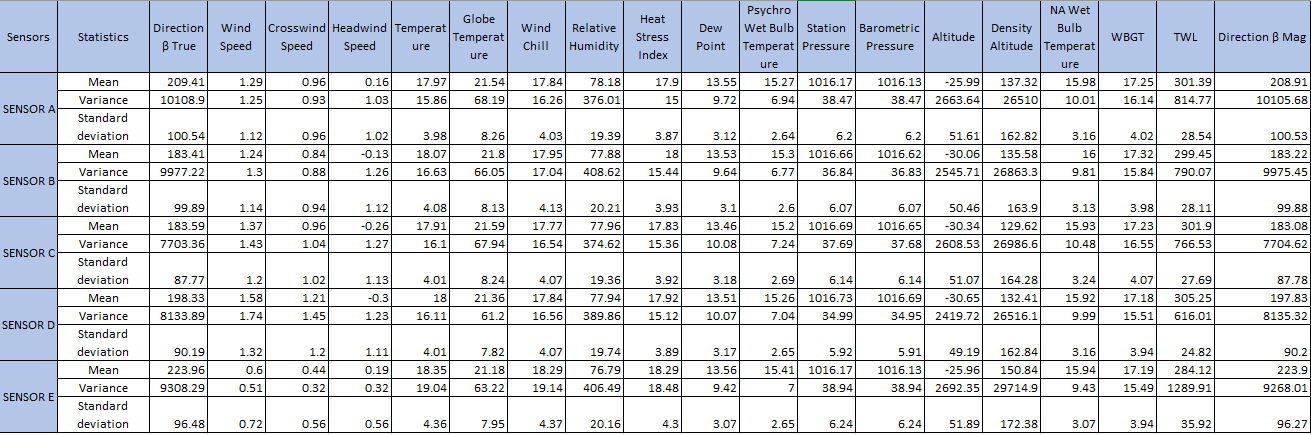
\includegraphics[width=0.9\textwidth]{Statistics_Matrix.png} 
	\caption{Mean,Variance and std of sensors variables} % Creates caption underneath graph
\end{figure}

Regarding the statistics results, there are not significant observations that can be made. There is not one sensor that has the highest or lowest results for every variable. In that case, further analysis is needed in order to make secure observations.

\subsection{Create 1 plot that contains histograms for the 5 sensors Temperature values. Compare histograms with 5 and 50 bins, why is the number of bins important?}

\begin{figure}[H] % places figure environment here   
	\centering % Centers Graphic
	\begin{subfigure}[b]{0.4\linewidth}
		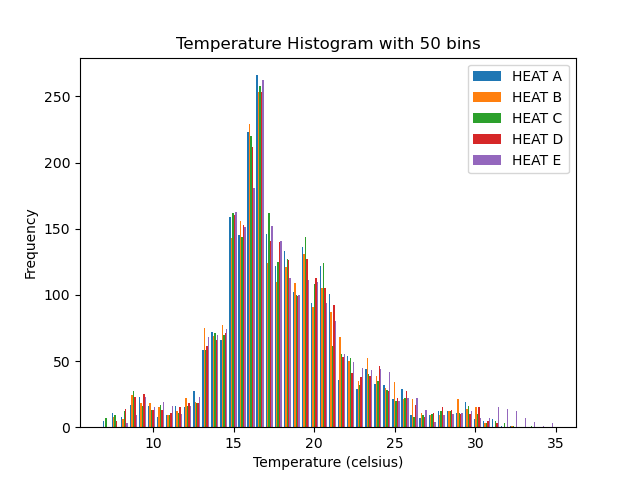
\includegraphics[width=0.9\linewidth]{Figure_1.png} 
		\caption{Temperature Histogram (50 bins)}
		\end{subfigure}
	\begin{subfigure}[b]{0.4\linewidth}
		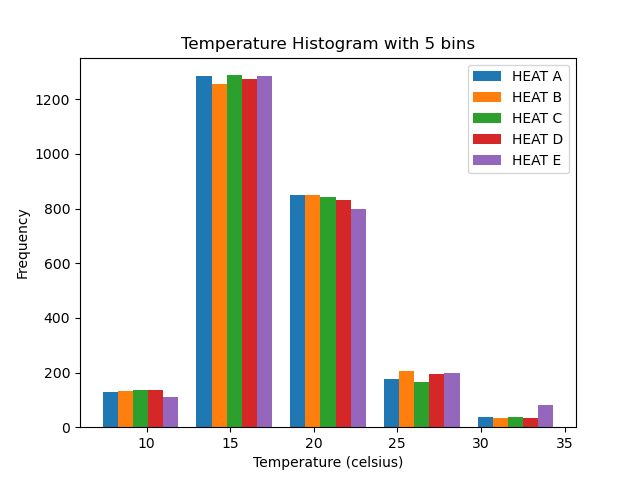
\includegraphics[width=0.9\linewidth]{Figure_2.png} 
		\caption{Temperature Histogram (5 bins)}
	\end{subfigure}
\end{figure}

The two figures above show the temperature histograms with 50 and 5 bins respectively. There are some significant differences between the 2 plots. The 50-bins histogram contains more detail than the 5-bins one. The minimum number of bins, in order to come to robust conclusions about the sample, can be calculated with Rice's rule.

\subsection {Create 1 plot where frequency polygons for the 5 sensors Temperature values overlap in different colors with a legend.}

\begin{figure}[H] % places figure environment here   
	\centering % Centers Graphic
	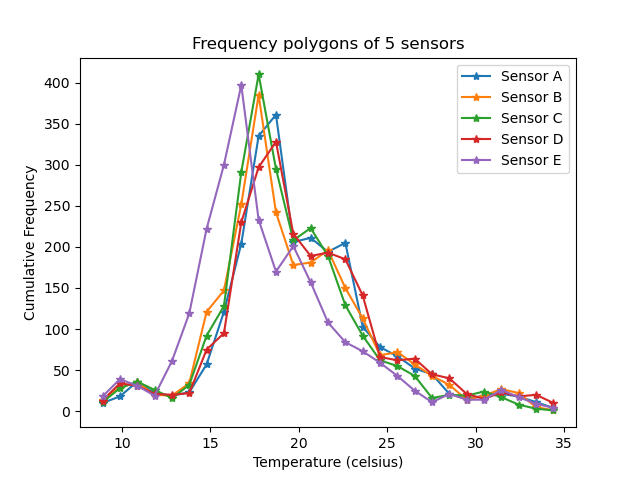
\includegraphics[width=0.9\textwidth]{Figure_3.png} 
	\caption{Frequency Polygons of 5 sensors} % Creates caption underneath graph
\end{figure}

In order to create the polygons, the number of bins was calculated with Rice's rule. The resulting number was 27.

\subsection {Generate 3 plots that include the 5 sensors boxplot for: Wind Speed, Wind Direction and Temperature.}

\begin{figure}[H] % places figure environment here   
	\centering % Centers Graphic
	\begin{subfigure}[b]{0.4\linewidth}
		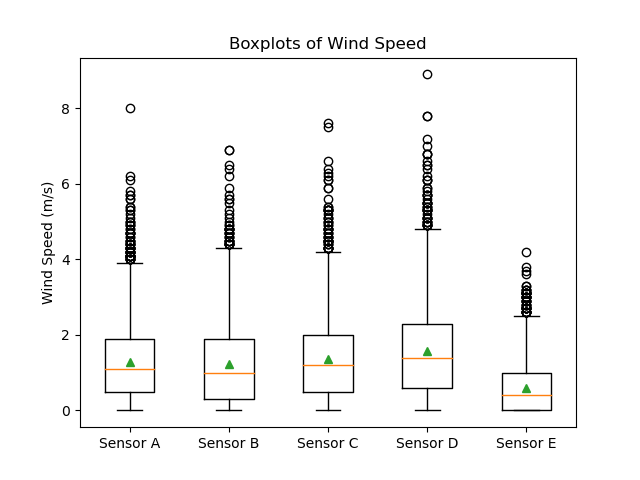
\includegraphics[width=0.9\linewidth]{Figure_4.png} 
		\caption{Boxplots of Wind Speed}
	\end{subfigure}
	\begin{subfigure}[b]{0.4\linewidth}
		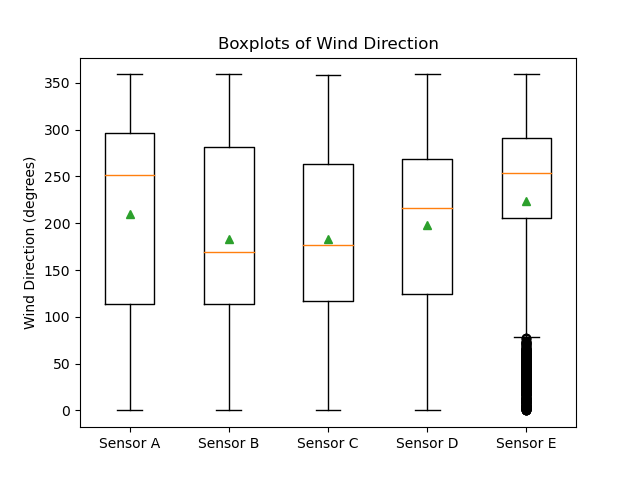
\includegraphics[width=0.9\linewidth]{Figure_5.png} 
		\caption{Boxplots of Wind Speed}
	\end{subfigure}
	\begin{subfigure}[b]{0.4\linewidth}
	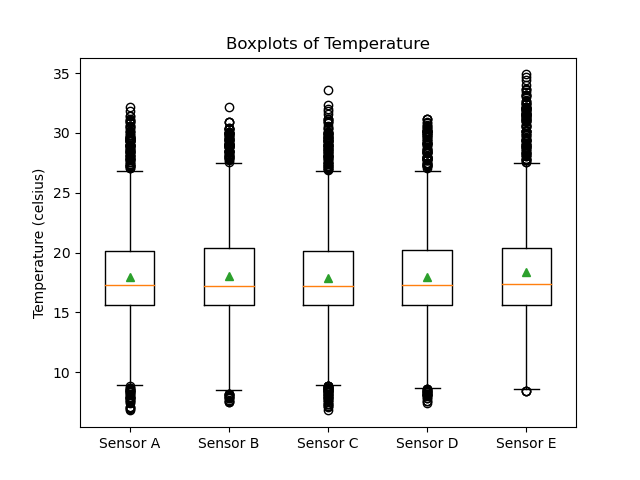
\includegraphics[width=0.9\linewidth]{Figure_6.png} 
	\caption{Boxplots of Wind Speed}
\end{subfigure}
\end{figure}

Each box represents a sensor.In total, three plots were created one for each variable. In the above figures a lot of outliers can be noticed in the Boxplot of Wind direction, for Sensor E.

\section{ Lesson A2}

\subsection{Plot PMF, PDF and CDF for the 5 sensors Temperature values in independent plots (or subplots). Describe the behavior of the distributions, are they all similar? what about their tails?}

\begin{figure}[H] % places figure environment here   
	\centering % Centers Graphic
	\begin{subfigure}[b]{0.4\linewidth}
		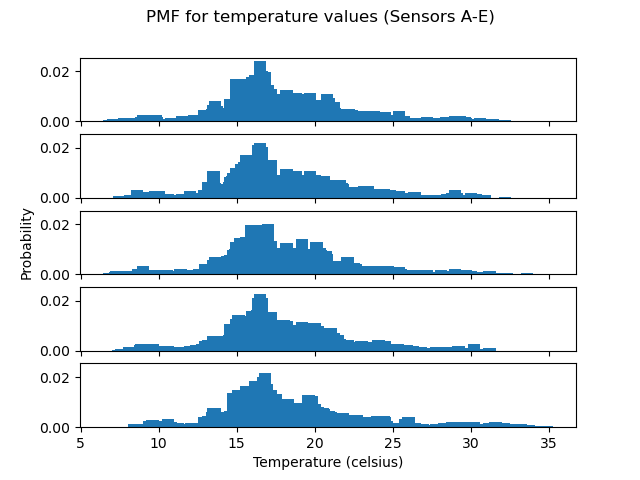
\includegraphics[width=0.9\linewidth]{Figure_7.png} 
		\caption{PMF for Temperature values}
	\end{subfigure}
	\begin{subfigure}[b]{0.4\linewidth}
		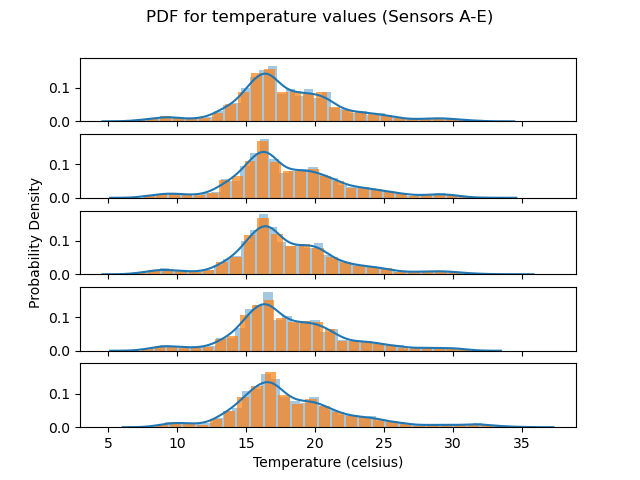
\includegraphics[width=0.9\linewidth]{Figure_8.png} 
		\caption{PDF for Temperature values}
	\end{subfigure}
	\begin{subfigure}[b]{0.4\linewidth}
		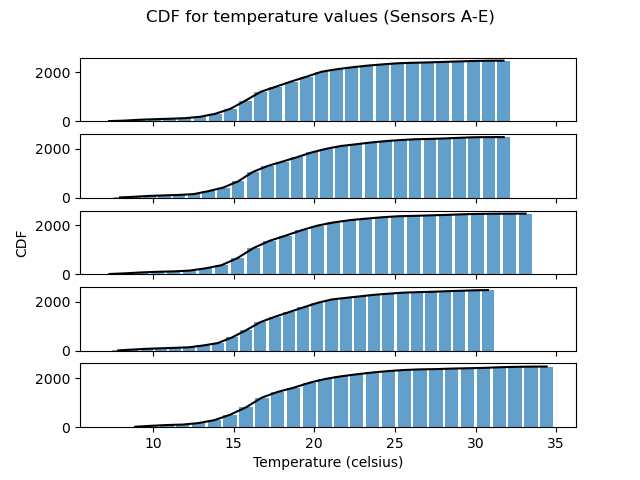
\includegraphics[width=0.9\linewidth]{Figure_9.png} 
		\caption{CDF for Temperature values}
	\end{subfigure}
\end{figure}

PMF and PPF seem to have similar distributions. Their peaks appear to be at 17-18 celsius, which is the mean temperature for all the sensors.On the other hand, CDF is a cumulative function that maps from a value to its percentile rank. That is why it is noticeable that the graph has higher y values from left to right. In all of the graphs though, temperature values of Sensor E appear to have bigger tails.


\subsection{For the Wind Speed values, plot the pdf and the kernel density estimation. Comment the differences.}

\begin{figure}[H] % places figure environment here   
	\centering % Centers Graphic
	\begin{subfigure}[b]{0.4\linewidth}
		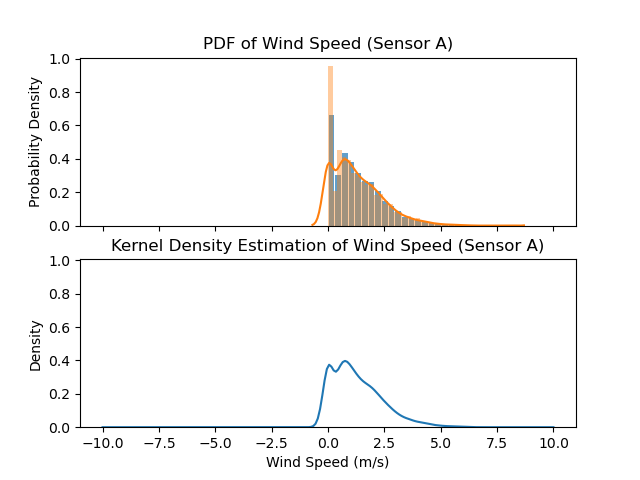
\includegraphics[width=0.9\linewidth]{Figure_10.png} 
		\caption{PDF and KDE for Wind Speed values (A)}
	\end{subfigure}
	\begin{subfigure}[b]{0.4\linewidth}
		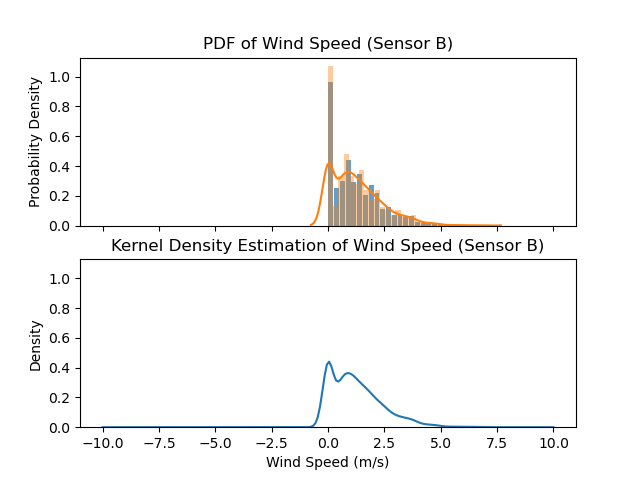
\includegraphics[width=0.9\linewidth]{Figure_11.png} 
		\caption{PDF and KDE for Wind Speed values (B)}
	\end{subfigure}
	\begin{subfigure}[b]{0.4\linewidth}
		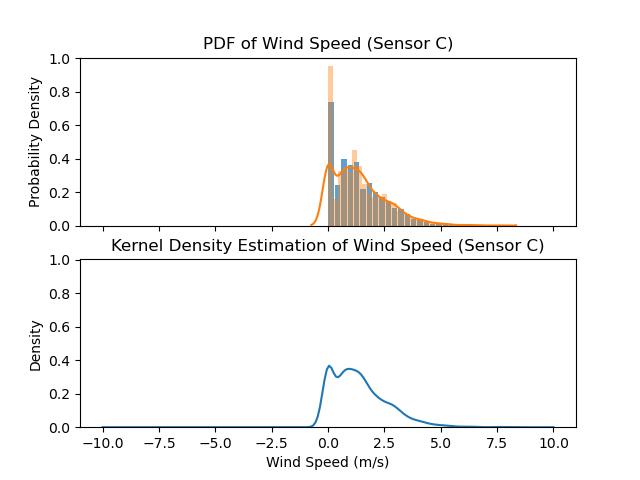
\includegraphics[width=0.9\linewidth]{Figure_12.png} 
		\caption{PDF and KDE for Wind Speed values (C)}
	\end{subfigure}
	\begin{subfigure}[b]{0.4\linewidth}
		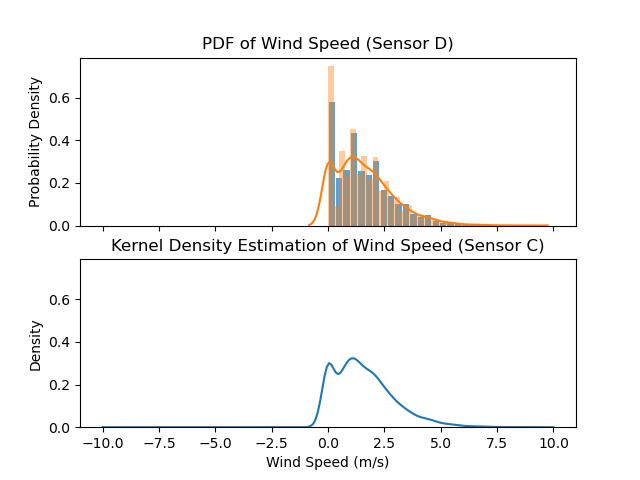
\includegraphics[width=0.9\linewidth]{Figure_13.png} 
		\caption{PDF and KDE for Wind Speed values (D)}
	\end{subfigure}
	\begin{subfigure}[b]{0.4\linewidth}
		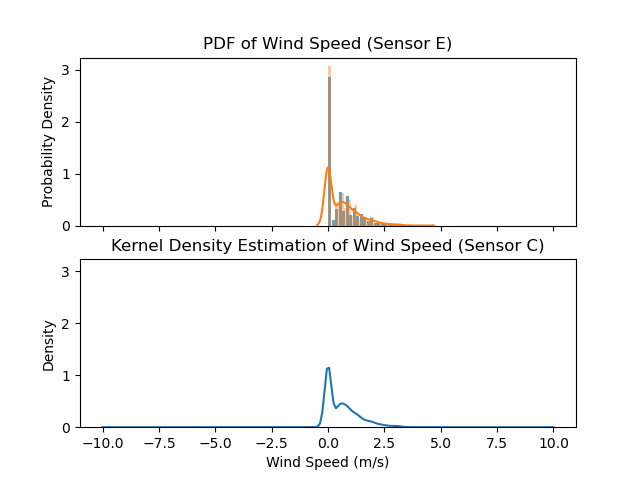
\includegraphics[width=0.9\linewidth]{Figure_14.png} 
		\caption{PDF and KDE for Wind Speed values (E)}
	\end{subfigure}
\end{figure}

In order to answer to this question, five figures were made, one for each sensor. There are two plots per figure, one representing the Probability Density Function and the other one the Kernel Density Estimation for the wind speed values. The two graphs are not the same but they have minor differences in each sensor. This result has a logical explanation, because  KDE is an algorithm that takes a sample and finds an appropriately smooth PDF that fits the data. 

\section{ Lesson A3}

\subsection{Compute the correlations between all the sensors for the variables: Temperature, Wet Bulb Globe Temperature (WBGT), Crosswind Speed. Perform correlation between sensors with the same variable, not between two different variables; for example, correlate Temperature time series between sensor A and B. Use Pearson’s and Spearmann’s rank coefficients. Make a scatter plot with both coefficients with the 3 variables.}

\begin{figure}[H] % places figure environment here   
	\centering % Centers Graphic
	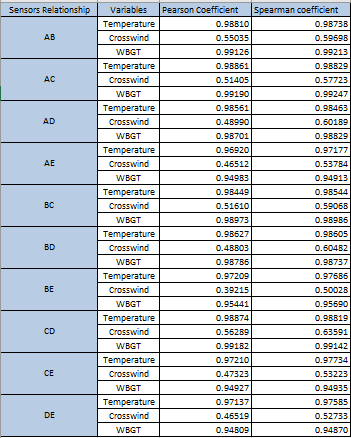
\includegraphics[width=0.9\textwidth]{Coefficients.png} 
	\caption{Pearson and Spearmann Correlation between the sensors} % Creates caption underneath graph
\end{figure}

\begin{figure}[H] % places figure environment here   
	\centering % Centers Graphic
	\begin{subfigure}[b]{0.4\linewidth}
		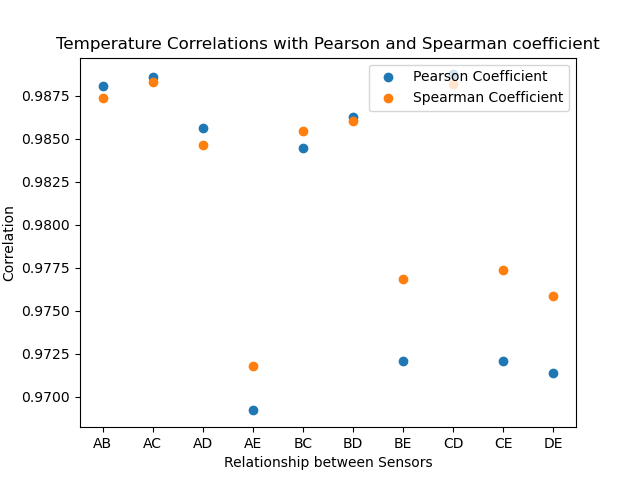
\includegraphics[width=0.9\linewidth]{Figure_15.png} 
		\caption{Temperature correlation between sensors}
	\end{subfigure}
	\begin{subfigure}[b]{0.4\linewidth}
		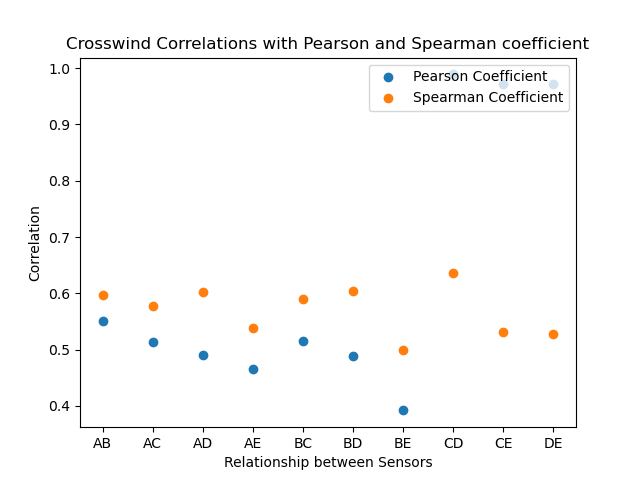
\includegraphics[width=0.9\linewidth]{Figure_16.png} 
		\caption{Crosswind correlation between sensors}
	\end{subfigure}
	\begin{subfigure}[b]{0.4\linewidth}
		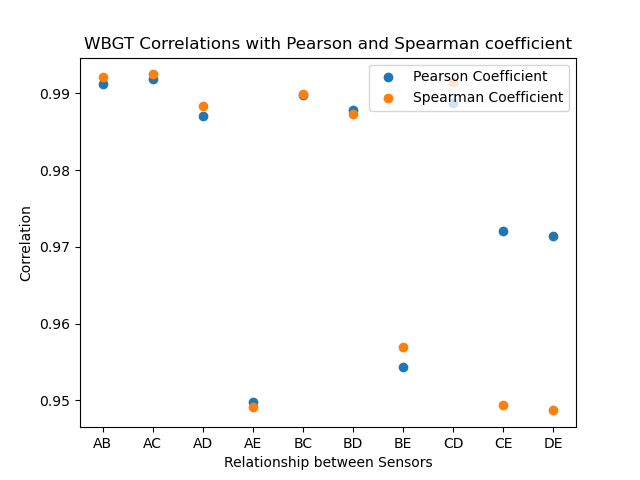
\includegraphics[width=0.9\linewidth]{Figure_17.png} 
		\caption{WBGT correlation between sensors}
	\end{subfigure}
\end{figure}

\subsection{What can you say about the sensors’ correlations?}

By comparing the matrix and the scatter plots, some results on the sensors' correlations can be presented. First of all, the correlation values from the Crosswind data are lower, close to 0.5, compared to the ones produced by the other two variables.In the Temperature and WBGT plots all the sensors have very high correlations between each other. There are differences between Pearson and Spearman Coefficients, a fact that is caused due to their different abilities in expressing linear and non-linear information. It is detectable that in all the plots, Sensor E involved in the lowest correlations.

\subsection{If we told you that that the sensors are located as follows, hypothesize which location would you assign to each sensor and reason your hypothesis using the correlations.}

\begin{figure}[H] % places figure environment here   
	\centering % Centers Graphic
	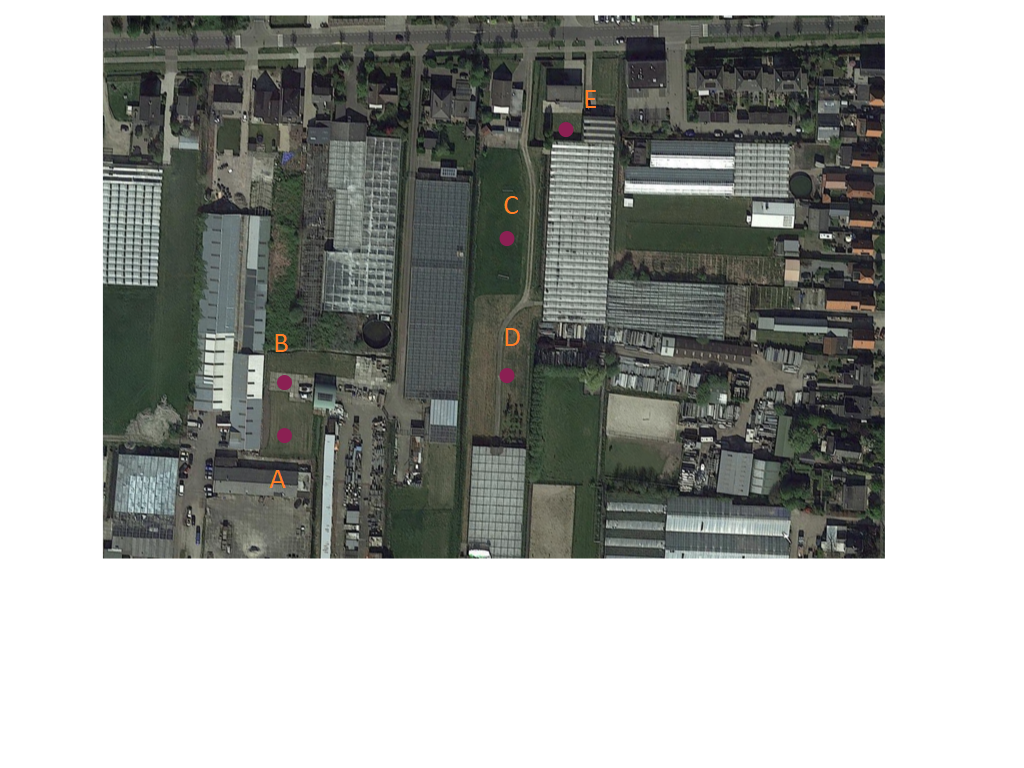
\includegraphics[width=0.9\textwidth]{SensorsSketch.png} 
	\caption{Sensor Map} % Creates caption underneath graph
\end{figure}

Depending on the correlation values between the sensors, as well as the scatter plots, some conclusions were made.After the creation of some scatter plots for the three variables,it was found that the temperature and WBGT correlations were linear, while the scatter plot of croswind was non linear. That is the reason, the Spearman Coefficient was prefered in order to justify the location of the sensors based on crosswind. First of all, in my opinion Sensor E is on the northeast side of the map as shown above. This conclusion was made, due to the fact that E has the lowest correlations with the other sensors. From the location of the sensor, it can be observed that it is surrounded by buildings,in contrast to the other locations, which may explain the low correlation regarding windspeed. Moreover, next to it Sensor C was placed, due to the fact that it has the least worse correlations to Sensor E, comparing to the other sensors. South of C, Sensor D was assigned,because these 2 sensors have the best correlations in terms of WindSpeed and Temperature. Their location is close, they seem to be based on the same type of soil and surrounded by the same buildings. West of D, Sensor B was assigned because comparing to A it is better correlated to D, in  terms of all the variables.In the end, Sensor A was placed in the southwestern part, because it is really close to B and also surrounded by the same buildings, a conclusion that can be made due to their high correlations in the three variables.

\section { Lesson A4}

\subsection{Plot the CDF for all the sensors and for variables Temperature and Wind Speed, then compute the 95 confidence intervals for variables Temperature and Wind Speed for all the sensors and save them in a table (txt or csv form).}

\begin{figure}[H] % places figure environment here   
	\centering % Centers Graphic
	\begin{subfigure}[b]{0.4\linewidth}
		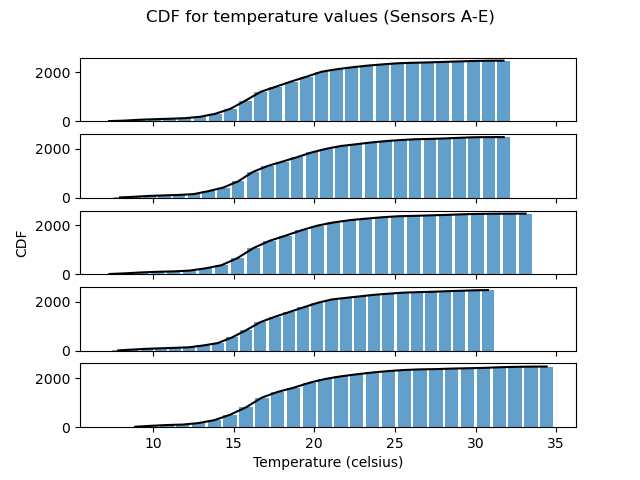
\includegraphics[width=0.9\linewidth]{Figure_9.png} 
		\caption{CDF for Temperature values}
	\end{subfigure}
	\begin{subfigure}[b]{0.4\linewidth}
		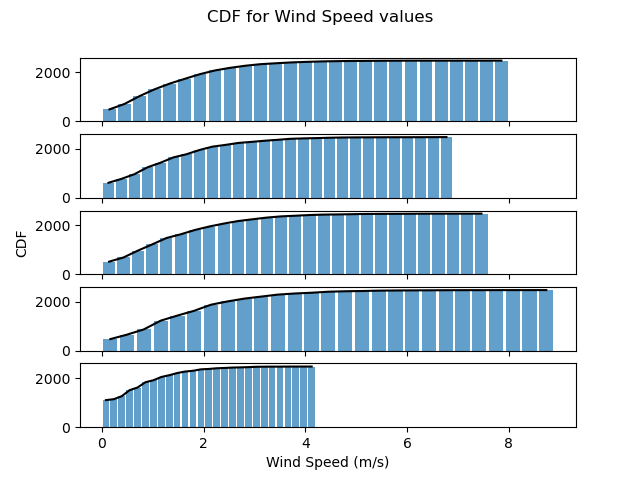
\includegraphics[width=0.9\linewidth]{Figure_18.png} 
		\caption{CDF for Wind Speed values}
	\end{subfigure}
\end{figure}

It is noticeable that Sensor E has the biggest tail for Temperature values. At the same time, it appears to have the shortest one for Wind speed.

\begin{figure}[H] % places figure environment here   
	\centering % Centers Graphic
	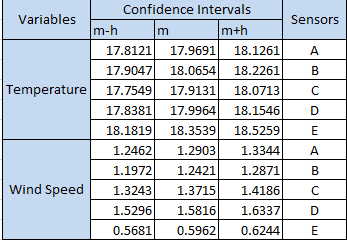
\includegraphics[width=0.5\textwidth]{Confidence_intervals.png} 
	\caption{Confidense intervals between Sensors} % Creates caption underneath graph
\end{figure}

\subsection{Test the hypothesis: the time series for Temperature and Wind Speed are the same for sensors:1) E, D 2) D, C 3) C, B; 4) B, A. What could you conclude from the p-values?}

\begin{figure}[H] % places figure environment here   
	\centering % Centers Graphic
	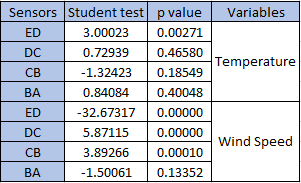
\includegraphics[width=0.5\textwidth]{T_test.png} 
	\caption{Student test and p-values} % Creates caption underneath graph
\end{figure}

The hypothesis for the requested sensors was made and the results can be seen above. In order to understand the significance of p-values, a null hypothesis was suggested, that the sensors mentioned above have the same Temperature and Windspeed values. Low p-values indicate that the effect is said to be statistically
significant, which means that it is unlikely to have occurred by chance. In that case, the null hypothesis is invalid. The lowest values are observed between Sensors E and D, as well as D and C and they are very close to 0.

\section {Bonus question}

\subsection {Your “employer” wants to estimate the day of maximum and minimum potential energy consumption due to air conditioning usage. To hypothesize regarding those days, you are asked to identify the hottest and coolest day of the measurement time series provided. How would you do that? Reason and program the python routine that would allow you to identify those days.}

For the following question the hottest and coolest days per sensor were calculated. In order to achieve that, a function in python was created, entitled as average temperature that took one variable which was the data. The function contains two lists, one named "temperature" and the other one "dates". The first list reads the temperature data from the excel files \cite{Maiullari2020}. Every day there were 72 measurements, every 20 minutes. So, the mean temperature for each day was calculated. The second list includes the strings of the dates, that measurements took place. Furthermore, a dataframe including those two lists was created and then it was sorted from the hottest to the coolest temperature.Then the function prints the hottest and coolest values and the corresponding dates. Last but not least, outside the function, five print statements were coded, so that the results for each sensor can be seen. The results can be seen below:

\begin{figure}[H] % places figure environment here   
	\centering % Centers Graphic
	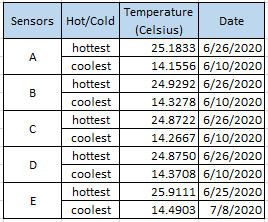
\includegraphics[width=0.5\textwidth]{Bonus.png} 
	\caption{Highest and lowest temperatures per sensor} % Creates caption underneath graph
\end{figure}

For sensors A-D the hottest day is 26/6/2020, while the coolest day 10/6/2020. The difference appears in Sensor E, where the hottest day is 25/6/2020 and the coolest on 8/7/2020.

\bibliographystyle{plain}
\bibliography{bibliography}
\end{document}
